\chapter{Correctness}
\label{chap:correctness}

The Meteor authors have released a demo of Meteor at \cite{MeteorDemo2021}. On the website, they state that ``due to issues with the GPT-2 algorithm interface, you sometimes may see extra output from a decoded stegotext. This does not impact the underlying security of the scheme''.
During experimentation,  we have concluded that the cause of this is due to the way subword based GNNs, such as GPT-2, encode text and not due to issues with the algorithm interface.

In this chapter, we will, after describing the issue at hand, show that the Meteor Stegosystem is indeed incorrect with respect to Hopper's definition as defined in \autoref{def:correctness-hopper} by providing a counterexample.
Afterwards, an experiment will be presented which has been performed to approximate the probability of incorrect decodings.
The experiment shows that for sufficiently long hiddentexts the probability of incorrect decoding increases to about 82 \%.
To restore correctness, we concludingly present a change to Meteor's $Decoder$ algorithm to increase the probability of successfully recovering the hiddentext message while introducing overhead exponential in stegotext length.

\section{Ambiguous Tokenization}

In \autoref{sec:generative-neural-networks}, we discuss that GPT-2 uses a token dictionary to represent text.
To improve generated text quality, modern GNNs use subword tokens.
Subword tokenization is opposed to word tokenization, where text is split by spaces, and character-based tokenization, which tokenizes text character by character.
Subword tokenization allows for more effective deep learning, as the model can easier connect related words to each other. 
For example, the model might learn that, by adding the suffix ``n't'' to a verb, one can invert the meaning of that verb, e.g. ``haven't'' is the opposite of ``have''.
This technique proved to be very effective in enhancing GNN performance in the last few years.

On the other hand, this allows for one word to have multiple representations in the ML model.
For example, the word ``doesn't'' might be tokenized by a tokenizer $T$ over tokens $\mathcal{T}$ as $T(\textrm{``doesn't''}) = ( \textrm{``do''}, \textrm{``es''}, \textrm{``n't''} )$.
It could also be tokenized as $T(\textrm{``doesn't''}) = ( \textrm{``does''}, \textrm{``n't''} )$ or even $T(\textrm{``doesn't''}) = ( \textrm{``d''}, \textrm{``o''}, \textrm{``e''}, \textrm{``s''}, \textrm{``n''}, \textrm{``'t''})$.
This situation is what we call an ambiguous tokenization.

We define a distance function $D$ between tokenizations from Alice and Bob as the following:

\begin{definition}[Tokenization Distance]
Let $t, t' \in \mathcal{T}^*$ be sequences of tokens.
We define the \emph{tokenization distance between t and t'} with a function $D \colon \mathcal{T}^* \times \mathcal{T}^* \rightarrow \mathbb{N}$ as

$$D(t, t') = \left| \left\{ i \in [1, |t|] \mid \exists i' > 1~ \exists l > 0: t_{i-1} = t'_{i'-1} \land \left( \bigwedge_{j=0}^{l-1} t_{i+j} \neq t'_{i'+j} \right) \land t_{i+l} = t'_{i'+l} \right\} \right|$$
\end{definition}

This distance function is a measure for the number of tokenization mismatches between the sending party Alice and the receiving party Bob.
We denote the function $T_P \colon \Sigma^* \rightarrow \mathcal{T}^*$ as the tokenizer used by party $P$ to generate or parse the stegotext $s \in \Sigma^*$.

\begin{example}
Let $s = \textrm{``hello''}$ be a text generated by sending party Alice with tokenization $T_A(s) = (\textrm{``he''}, \textrm{``llo''})$.
Let $T_B(s) = (\textrm{``he''}, \textrm{``l''}, \textrm{``lo''})$ be the tokenization of $s$ generated by the receiving party Bob.
The distance between $T_A(s)$ and $T_B(s)$ is 

$$
D(T_A(s), T_B(s)) 
= D( (\textrm{``he''}, \textrm{``llo''}), (\textrm{``he''}, \textrm{``l''}, \textrm{``lo''})  ) 
= \left| \left\{ 2 \right\} \right| = 1
$$
\end{example}


\todo{double check if D is correct}



%\begin{definition}[Ambiguous Tokenization]
%	\label{def:amb-tok}
%	Let $\mathcal{M}$ be a GNN with tokens $\mathcal{T} = \{ t_1, t_2, \dots, t_n \}$.
%	We say that $\mathcal{M}$ has an ambiguous tokenization, if there exists at least two lists of indices $X = (i, j, k, \dots), Y = (q, r, s, \dots), X \neq Y$ with $T_X = t_i || t_j || t_k || \dots$ and $T_Y = t_q || t_r || t_s || \dots$ such that $T_X = T_Y$.
%\end{definition}

\section{Correctness Of The Meteor Stegosystem}

In \autoref{alg:decode}, we see that during decoding, the stegotext $c$ generated by \autoref{alg:encode} should be parsed as $c = c_0 ||c_1 || \dots || c_{\tau}$.
This task is performed by a tokenizer over tokens $\mathcal{T}$ specific to the underlying model.
Meteor's decode algorithm expects that the parsing of $c$ can recover the $c_i$ originally generated during encoding.
This unfortunately is, at least for models with subword tokenizations such as GPT-2, not the case for some combinations of stegotext, key and history due to ambiguous tokenization as defined above.
In \autoref{sec:alg-rec-tok-candidates}, we will show how to fix these correctness issues.

\begin{theorem}
The Meteor Stegosystem is not correct.
\end{theorem}

\begin{proof}
For Meteor to be correct, it must fulfil \autoref{def:correctness-kaptchuk}, i.e. for any $k \leftarrow KeyGen(1^\lambda)$, hiddentext $m$ and history $h$:

$$\mathop{Pr}[Decode_{\mathcal{D}}(k, Encode_{\mathcal{D}}(k, m, h), h) = m] \geq 1 - \mu(\lambda)$$

We show incorrectness by giving a counterexample. 
The counterexample below has been generated by repeatedly encoding a fixed message and history using the Meteor stegosystem with random keys.
We will later show that the encoding fails for many or most keys $k$, especially if the encoded messages $m$ are long ($|m| \geq 1024$ bytes).
Let

\begin{lstlisting}[breaklines]
k = 0xb95e03a1d01b304f11dcf2bc844e5fd3cbed41253b0506876004207b2c2a10e
    2d89c1a40e93530bfcfaaee54e66ae048d2d2a536615b0a81afe792883877d5b6
m = 'Hello world'
H = 'Despite a long history of research and wide-spread applications to censorship resistant systems, practical steganographic systems capable of embedding messages into realistic communication distributions, like text, do not exist.\n\n'
\end{lstlisting}

The stegotext for these inputs when using the Meteor demo code at \cite{MeteorDemo2021} is

\begin{lstlisting}
c = '\nZeus communication system, controlled by anÆ2 desktop mic with'
\end{lstlisting}

When passed to the standard GPT-2 Tokenizer, the substring ``Zeus'' of $c$ is parsed as \lstinline{['Z', 'eus']}, while the encoding process has generated ``Zeus'' with token sequence \lstinline{['Ze', 'us']}.
Therefore, the stegotext $c$ cannot be successfully decoded to the original hiddentext ``Hello world'', which violates correctness.
\end{proof}

After we have seen that this problem appears at least once by finding a counterexample, another question arises:
How often does this happen?
If this happens only for a negligible amount of combinations of message, key, and history (or maybe even only for this exact combination), this might be a non-issue.

To approach this question, we first define a random variable $X$ as the distance between token sequences $T_A(s)$ and $T_B(s)$ generated by Alice and Bob respectively for a stegotext $s = Encode_{\mathcal{D}}(k,m,h) \in \Sigma^*$:

$$Pr[X=a] = \frac{\left| \left\{ s \in \Sigma^* \mid D(T_A(s), T_B(s)) = a \right\} \right|}{\left| \Sigma^* \right|}$$

As we have argued before, the decoding can only be successful if no tokenization mismatches appear, i.e. the tokenization generated by Alice and Bob are the same.
Thus, for a successful decoding, the distance between tokenizations must be zero.
We can establish the tokenization distance as an upper bound for the decoding success:

$$Pr[Decode_{\mathcal{D}}(k, Encode_{\mathcal{D}}(k,m,h), h)=m] \leq Pr[X=0]$$

How can we determine the probability $Pr[X=0]$?
While there are exponentially many combinations of keys $k \in \{0,1\}^\lambda$ and histories $h \in \mathcal{H}$ (which we could potentially brute-force), there are infinitely many messages $m \in \{0,1\}^*$.
Therefore, we cannot determine $Pr$ exactly.
What we can do instead is fix some set of messages $K \subset \{0,1\}^\lambda$ for a fixed security parameter $\lambda$, $M_n \subset \{0,1\}^n$ of fixed length $n$ and $H \subset \mathcal{H}$ and calculate the distances $D$ for samples $(k,m,h) \in K \times M_n \times H$ to establish an approximation $\hat{Pr} \approx Pr$.

How do we select $K$, $M_n$ and $H$?
For $K$, we fix $\lambda = 512$ and uniformly choose random keys $k \leftarrow U_{512}$, for each sample $m \in M_n$.
For $M_n$, we use blocks of length $n=128$ or 1024 bytes from William Shakespeare's drama Hamlet, respectively.
The entire script of Hamlet is 191726 bytes long.
That gives us $|M_{128}|=\lceil \frac{191726}{128} \rceil = 1498$ and $|M_{1024}|= \lceil \frac{191726}{1024} \rceil = 188$ samples for $m$.
Even though the sample size for blocks of 1024 bytes is rather small, the average stegotext length grows proportionally to the number of bits encoded, so we can expect about the same length of token sequences for both experiments.
For $H$, we use random sequences from Hamlet of length 128 bytes for each sample $m \in M_n$.

After we have defined the sample data, we have encoded and subsequently decoded them using a modified version of the Meteor demo code from \cite{MeteorDemo2021}.
After decoding, we analyzed the tokens generated and compute the tokenization distance between the decoding and the encoding steps.

The experiment shows that most stegotexts have at least one mismatch if they are of significant length (\autoref{fig:meteor-stats-mismatch-count}).
When encoding 128 byte blocks, we get $\hat{Pr}[X=0] \approx 0.55$.
But when encoding larger blocks, that probability decreases to $\hat{Pr}[X=0] \approx 0.18$.

\begin{figure}[htbp]%
	\begin{subfigure}{.5\textwidth}%
		\centering%
	    \resizebox{0.9\linewidth}{!}{%
			% This file was created with tikzplotlib v0.10.1.
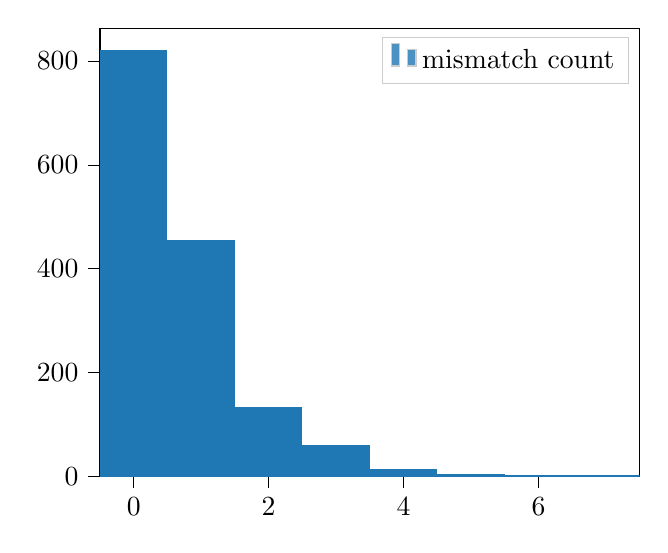
\begin{tikzpicture}

\definecolor{darkgray176}{RGB}{176,176,176}
\definecolor{lightgray204}{RGB}{204,204,204}
\definecolor{steelblue31119180}{RGB}{31,119,180}

\begin{axis}[
legend cell align={left},
legend style={fill opacity=0.8, draw opacity=1, text opacity=1, draw=lightgray204},
tick align=outside,
tick pos=left,
x grid style={darkgray176},
xmin=-0.5, xmax=7.5,
xtick style={color=black},
y grid style={darkgray176},
ymin=0, ymax=863.1,
ytick style={color=black}
]
\draw[draw=none,fill=steelblue31119180] (axis cs:-0.5,0) rectangle (axis cs:0.5,822);
\addlegendimage{ybar,ybar legend,draw=none,fill=steelblue31119180}
\addlegendentry{mismatch count}

\draw[draw=none,fill=steelblue31119180] (axis cs:0.5,0) rectangle (axis cs:1.5,455);
\draw[draw=none,fill=steelblue31119180] (axis cs:1.5,0) rectangle (axis cs:2.5,134);
\draw[draw=none,fill=steelblue31119180] (axis cs:2.5,0) rectangle (axis cs:3.5,61);
\draw[draw=none,fill=steelblue31119180] (axis cs:3.5,0) rectangle (axis cs:4.5,15);
\draw[draw=none,fill=steelblue31119180] (axis cs:4.5,0) rectangle (axis cs:5.5,5);
\draw[draw=none,fill=steelblue31119180] (axis cs:5.5,0) rectangle (axis cs:6.5,3);
\draw[draw=none,fill=steelblue31119180] (axis cs:6.5,0) rectangle (axis cs:7.5,3);
\end{axis}

\end{tikzpicture}
%
		}%
		\caption{128 bytes ($\hat{Pr}[X=0] \approx 0.55$)}%
	\end{subfigure}%
	\begin{subfigure}{.5\textwidth}%
		\centering%
	    \resizebox{0.9\linewidth}{!}{%
			% This file was created with tikzplotlib v0.10.1.
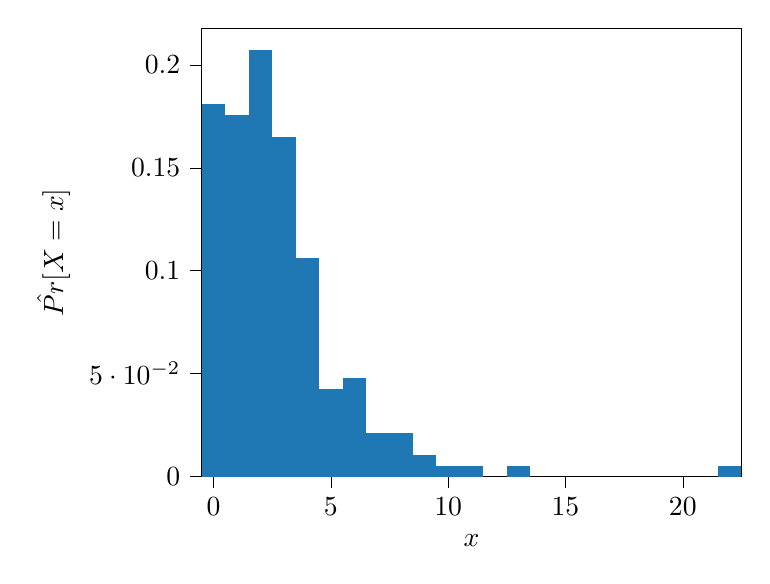
\begin{tikzpicture}

\definecolor{darkgray176}{RGB}{176,176,176}
\definecolor{steelblue31119180}{RGB}{31,119,180}

\begin{axis}[
tick align=outside,
tick pos=left,
x grid style={darkgray176},
xlabel={\(\displaystyle x\)},
xmin=-0.5, xmax=22.5,
xtick style={color=black},
y grid style={darkgray176},
ylabel={\(\displaystyle \hat{Pr}[X=x]\)},
ymin=0, ymax=0.21781914893617,
ytick style={color=black}
]
\draw[draw=none,fill=steelblue31119180] (axis cs:-0.5,0) rectangle (axis cs:0.5,0.180851063829787);
\draw[draw=none,fill=steelblue31119180] (axis cs:0.5,0) rectangle (axis cs:1.5,0.175531914893617);
\draw[draw=none,fill=steelblue31119180] (axis cs:1.5,0) rectangle (axis cs:2.5,0.207446808510638);
\draw[draw=none,fill=steelblue31119180] (axis cs:2.5,0) rectangle (axis cs:3.5,0.164893617021278);
\draw[draw=none,fill=steelblue31119180] (axis cs:3.5,0) rectangle (axis cs:4.5,0.106382978723405);
\draw[draw=none,fill=steelblue31119180] (axis cs:4.5,0) rectangle (axis cs:5.5,0.042553191489362);
\draw[draw=none,fill=steelblue31119180] (axis cs:5.5,0) rectangle (axis cs:6.5,0.0478723404255322);
\draw[draw=none,fill=steelblue31119180] (axis cs:6.5,0) rectangle (axis cs:7.5,0.021276595744681);
\draw[draw=none,fill=steelblue31119180] (axis cs:7.5,0) rectangle (axis cs:8.5,0.021276595744681);
\draw[draw=none,fill=steelblue31119180] (axis cs:8.5,0) rectangle (axis cs:9.5,0.0106382978723405);
\draw[draw=none,fill=steelblue31119180] (axis cs:9.5,0) rectangle (axis cs:10.5,0.00531914893617025);
\draw[draw=none,fill=steelblue31119180] (axis cs:10.5,0) rectangle (axis cs:11.5,0.00531914893617025);
\draw[draw=none,fill=steelblue31119180] (axis cs:11.5,0) rectangle (axis cs:12.5,0);
\draw[draw=none,fill=steelblue31119180] (axis cs:12.5,0) rectangle (axis cs:13.5,0.00531914893617025);
\draw[draw=none,fill=steelblue31119180] (axis cs:13.5,0) rectangle (axis cs:14.5,0);
\draw[draw=none,fill=steelblue31119180] (axis cs:14.5,0) rectangle (axis cs:15.5,0);
\draw[draw=none,fill=steelblue31119180] (axis cs:15.5,0) rectangle (axis cs:16.5,0);
\draw[draw=none,fill=steelblue31119180] (axis cs:16.5,0) rectangle (axis cs:17.5,0);
\draw[draw=none,fill=steelblue31119180] (axis cs:17.5,0) rectangle (axis cs:18.5,0);
\draw[draw=none,fill=steelblue31119180] (axis cs:18.5,0) rectangle (axis cs:19.5,0);
\draw[draw=none,fill=steelblue31119180] (axis cs:19.5,0) rectangle (axis cs:20.5,0);
\draw[draw=none,fill=steelblue31119180] (axis cs:20.5,0) rectangle (axis cs:21.5,0);
\draw[draw=none,fill=steelblue31119180] (axis cs:21.5,0) rectangle (axis cs:22.5,0.00531914893617025);
\end{axis}

\end{tikzpicture}
%
		}%
		\caption{1024 bytes ($\hat{Pr}[X=0] \approx 0.18$)}%
	\end{subfigure}%
	\caption{
	Token mismatch count statistics when using Meteor to encode Shakespear's Hamlet blockwise for different block sizes.
	We denote the random variable $X$ as the number of encoding mismatches in a stegotext.
	The x-axis shows the number of tokenization mismatches between the encoding and the decoding party for hiddentext blocks of size...}
	\label{fig:meteor-stats-mismatch-count}	
\end{figure}

%In the same experiment, we have also measured the mismatch length, which is the number of tokens which have to be skipped in the stegotext to get back in sync with the decoding party.
%For example, if a stegotext ``steganography is great'' was encoded with token sequence (steg, ano, graphy, \verbvisiblespace is, \verbvisiblespace great), but decoded as (ste, ga, no, graphy, \verbvisiblespace is, \verbvisiblespace great), the mismatch length is two, because the two tokens \emph{steg} and \emph{ano} have to be skipped on the encoded token sequence to get back in sync between encoding and decoding party when encounterint the token \emph{graphy}
%This measure will later help us estimate how far we should look ahead in the stegotext when trying to recover from decoding errors.

%\begin{figure}[htbp]%
%	\begin{subfigure}{.5\textwidth}%
%		\centering%
%	    \resizebox{0.8\linewidth}{!}{%
%			\input{fig_meteor_stats_mismatch_length_128.tikz}%
%		}%
%		\caption{128 bytes}%
%	\end{subfigure}%
%	\begin{subfigure}{.5\textwidth}%
%		\centering%
%	    \resizebox{0.8\linewidth}{!}{%
%			\input{fig_meteor_stats_mismatch_length_1024.tikz}%
%		}%
%		\caption{1024 bytes}%
%	\end{subfigure}%
%	\caption{
%	Token mismatch length statistics when using Meteor to encode Shakespear's Hamlet blockwise for different block sizes.
%	The x-axis shows the lengths of tokenization mismatches of the decoding party for hiddentext blocks of size...}
%	\label{fig:meteor-stats-mismatch-count}	
%\end{figure}

Therefore, we have to find a way to deal with these failed decodings, especially if we plan to encode hiddentext messages of significant length such as HTTP messages or Diffie-Hellman key exchange messages.
In \autoref{sec:alg-rec-tok-candidates}, we will present an approach to recover from decoding errors while introducing computational overhead exponential in stegotext length. 
In \autoref{chap:twowaycommunication}, we will show how we can split the hiddentext message and use Microsoft's DialoGPT -- a derivation of GPT-2 -- to generate chat-like stegotext.
Splitting the hiddentext results in shorter stegotext and thus decreases the probability of tokenization mismatches.



\section{Algorithmic Reconstruction Of Token Candidates}
\label{sec:alg-rec-tok-candidates}

Unfortunately, with subword tokenization, the decoding party cannot decide which tokens have been sampled to generate a given stegotext.
To allow successful decoding of ambiguously tokenized stegotexts, we will introduce algorithms to detect and fix wrong tokenizations.


For that we have to modify the encoding step of Meteor to detect and fix wrong tokenization.
Before encoding, split the message $m$ into blocks $m_i$ of length $\gamma$. \todo{variable block length?}
After each block $m_i$, add another block $q_i = q(m_i)$ of length $\delta$ into the hiddentext, i.e. $q \colon \{ 0,1 \}^\gamma \rightarrow \{ 0,1 \}^\delta$.
This value helps the decoder to decide if the decoding is still correct up to this point.
The block $q_i$ can be a checksum of $m_i$ or a fixed marker.
By adding checksums, we introduce $\delta \cdot \frac{|m|}{\gamma}$ bits of overhead to the hiddentext.
The modified $Encode$ algorithm can be found in \autoref{alg:marked-encode}.

Now the decoding party has to verify that after each block $m_i$ of $\gamma$ bits, the marker $q(m_i)$ appears and is valid.
If not, a decoding error has occured in the stegotext, i.e. a tokenization mismatch has been occured.
To recover from this, the decoding party has to roll back their encoding and generate all possible tokenizations since their last successful checksum check.
When they find a tokenization with correct checksum, the decoder expects that the correct tokenization has been found and proceeds.

It is still possible that a wrong tokenization randomly yields a correct checksum.
In an actual implementation, one might want to check multiple blocks in advance before expecting that the correct tokenization has been found.
The amount of blocks which should be checked to be sufficiently confident that the correct tokenization has been found primarily depends on block length $\gamma$ and checksum length $\delta$.
Determining specific values for $\gamma$ and $\delta$ is a trade-off between stegotext length and computational overhead in the case of a decoding error.
While longer checksums $\delta$ decreases the risk of falsely verified checksums, longer checksums causes longer stegotexts.
If we chose $\gamma = |m|$, only one checksum is generated over the entire message. If an error is detected after decoding the entire hiddentext, every possible tokenization for the stegotext $s$ has to be generated, which are exponential in stegotext length.
If we choose a small $\gamma$, many checksums are inserted, increasing stegotext length.
A modified $Decode$ algorithm can be found in \autoref{alg:marked-decode}.

\begin{Pseudocode}[caption={
Marked Encode Algorithm.
The modification this algorithm introduces is that after every $\gamma$ bits a checksum $q(m_i)$ is inserted into the hiddentext.
This allows the recipient to check for decoding errors due to wrong tokenization.
$q$ is a function $q \colon \{0,1\}^\gamma \rightarrow \{0,1\}^\delta$ which generates a checksum of length $\delta$ for a message block of length $\gamma$.
}, label={alg:marked-encode}]
algorithm $MarkedEncode_{\mathcal{M}}^{\beta, \gamma, \delta}(k_{prg}, m, h, q)$
	Output: Stegotext message $c$
	$c \leftarrow \epsilon,~ n \leftarrow 0,~ m^* \leftarrow \epsilon,~ j \leftarrow 0$
	while $j < |m|$ do
		$m^* \leftarrow m^* || m_j$
		$j \leftarrow j + 1$
		if $j \equiv 0~ \pmod \gamma$
			$m^* \leftarrow m^* || q(m_j)$
	while $n < |m^*|$ do
		$mask \leftarrow PRG.Next(k_{prg})$
		$r \leftarrow m^*[n:n+\beta] \oplus mask$
		$c_i \leftarrow Sample_{\mathcal{M}}^\beta(h, r)$
		$\mathcal{R} = Recover_{\mathcal{M}}^\beta(h, c_i)$
		$n_i \leftarrow LenPrefix^\beta(\mathcal{R})$
		$c \leftarrow c || c_i, n \leftarrow n+n_i, h \leftarrow h||c_i$
	Output $c$
\end{Pseudocode}



\begin{Pseudocode}[caption={
Marked Decode Algorithm.
In comparison to Meteor's $Decode$ algorithm, MarkedDecode checks the checksum every $\gamma$ bits. 
If the checksum does not match, a decoding error happened.
We then perform a lookbehind on the stegotext and generate all possible tokenizations $paths$ for a substring of $c$.
Afterwards, rewind the internal state and retry decoding with a path $p$ selected from $paths$.
}, label={alg:marked-decode}]
algorithm $MarkedDecode_{\mathcal{M}}^{\beta,\gamma,\delta}(k_{prg}, c, h, q)$
	Output: Plaintext message $m$
	$m^* \leftarrow \epsilon,~ n \leftarrow 0,~ j \leftarrow 0,~ i^* \leftarrow 0,~ s \leftarrow 0$
	$paths \leftarrow \emptyset$
	Parse $c$ as $c_0 || c_1 || \dots || c_{\tau}$
	for $i \in \{ 0, 1, \dots, \tau \}$ do
		$\mathcal{R} = Recover_{\mathcal{M}}^\beta(h, c_i)$
		$n_i \leftarrow LenPrefix^\beta(\mathcal{R})$
		$n \leftarrow n + n_i$
		$j \leftarrow j + n_i$
		$m_i \leftarrow Prefix^\beta(\mathcal{R})$
		$mask \leftarrow PRG.Next(k_{prg})$
		$m^* \leftarrow m^* || (m_i \oplus mask[0: |m_i|])$
		$h \leftarrow h||c_i$
		if $j \geq \gamma + \delta$
			# calculate checksum
			$j \leftarrow j \mod (\gamma+\delta)$
			if $m^*[s+\gamma:s+\gamma+\delta] \neq q(m^*[s:s+\gamma])$  # checksum failed
				$j^* \leftarrow \min_{a \in \{ i^*, \dots, \tau \}} (c[a] = \textrm{'~ '})$
				$c^* \leftarrow c_{i^*} || c_{i^*+1} || \dots || c_{j^*-1}$
				if $paths = \emptyset$
					$paths \leftarrow AllPaths(TokenizeCandidates_{\mathcal{T}}(c^*), c^*)$
				$p \leftarrow SelectPath_{\mathcal{M}}(paths, h)$
				replace $c_i^*||c_{i^*+1}||\dots||c_{j^*-1}$ with $p$
				rewind PRG state and variables to state at $i^*$
				retry decoding of $m^*[s:|m^*|]$ with $p$
			else  # checksum ok, expect first $i$ tokens to be correctly decoded
				$paths \leftarrow \emptyset$
				$s \leftarrow s + \gamma + \delta$
				$i^* \leftarrow i$
	$j \leftarrow 0$
	$m \leftarrow \epsilon$
	while $j < |m|$ do  # remove checksums from $m^*$
		$m \leftarrow m^* || m^*[j: j + \gamma]$
		$j \leftarrow j + \gamma + \delta$
	Output $m$
\end{Pseudocode}
\todo{parse $m$ as $m_1||q_1||m_2||q_2||\dots||m_\xi||q_\xi$}
\todo{MarkedDecode: $c_{i^*+x}$ explain $c^*$ length}
\todo{fix MarkedDecode}

For the modifications in $MarkedDecode$, we need some helper algorithms to generate a graph representing all possible tokenizations, called $TokenizeCandidates$, for a given stegotext, generate $AllPaths$ in that graph, and $SelectPath$ from the generated paths.

We can represent the tokenization candidates in a graph using the ML model's tokens $\mathcal{T}$.
When passed a string $c$, the algorithm $TokenizeCandidates$ generates a directed, acyclic graph (DAG) $G = (V, E)$.
The nodes $v \in V$ represent all possible suffix strings of $c$ (including the empty string $\epsilon$) with $|V| = |c| + 1$.
The edges $e \in E$ represent possible tokens used to transition between suffixes.
An example graph for input ``hello'' can be found in \autoref{fig:ex-graph-tokenize-candidates}.
For example, ``hello'' can be transformed to ``lo'' with token ``hel''.

Now that we have a graph for $c$, we can generate every possible sequence of tokens which $c$ can be parsed as.
For that we use the algorithm $AllPaths$, which takes as inputs a graph $G = (V, E)$ and a start node $v_i \in V$ and returns a set of all possible paths between $v_i$ and a fixed sink $v_j = \epsilon$.

But how many paths exist between $v_i$ and $v_j$?
A path between two vertices is a subset of $E$ which contains both vertices.
In a maximum DAG, there are up to $2^{|V|-2} = 2^{|c|-1}$ subsets of $E$ which contain both $v_i$ and $v_j$.
Therefore, the output size of $AllPaths$ is, in the worst case, exponential in input length.
A DFS-based implementation for AllPaths can be found in \autoref{alg:all-paths}.

Remember that each path generated by $AllPaths$ is a possible tokenization of $c$.
To successfully decode the stegotext, we have to find the tokenization that has been used by the encoding party.

How can we select a tokenization from $paths$?
A simple strategy would be to choose one element at random and try to decode it.
If we encounter a checksum mismatch again, we select another until we have found the correct tokenization.
With this approach, we will find the correct tokenization on average after $\frac{|paths|}{2} \leq \frac{2^{|c|-1}}{2} = 2^{|c|-2}$ attempts.
For an implementation of $SelectPath$ which chooses a path at random refer to \autoref{alg:select-path-rnd}.

While there are more advanced strategies to select a tokenization, e.g. by selecting a tokenization according to the probability distribution generated by the ML model, this simple approach is still viable when using the english language since we only generate paths for single words with relative short lengths.
As has been shown in \cite{BoShSo2012} by analyzing books from different epochs, the average word length in the english language is about five characters.
Therefore, an average english word can have up to $2^4 = 16$ possible tokenizations.
There still are commonly used (and therefore generated) words with a length of up to 13 characters such as ``international'' or ``circumstances'', which could have up to $2^{12} = 4096$ possible tokenizations.
Our experiments have shown that when using the GPT-2 tokenizers, the graphs for common longer words of the english language are still relatively small with less than $2^{11}$ possible paths.



\begin{Pseudocode}[float,caption={
TokenizeCandidates Algorithm.
This generates a graph $G = (V, E)$ from a string $c$.
Vertices are substrings of $c$, each edge represents a token to use to transform between substrings.
}, label={alg:tokenize-candidates}]
algorithm $TokenizeCandidates_{\mathcal{T}}(c)$
	Output: Graph $G = (V, E)$
	if $s = \epsilon$
		return $(\emptyset, \emptyset)$
	for $t \in \{ t' \in \mathcal{T}~ |~ t' \textrm{ is prefix of } s \}$ do
		$V \leftarrow V \cup \{ s[|t|{:}] \}$
		$E \leftarrow E \cup \{ (s, s[|t|{:}]) \}$
		$G \leftarrow G \cup TokenizeCandidates_{\mathcal{T}}(s[|t|{:}])$
	return $G$
\end{Pseudocode}

\begin{figure}[htbp]
	\centering
	\begin{tikzpicture}
		\node[block] (hello) {hello};
		\node[block, right=15mm of hello] (lo) {lo};
		\node[block, above=15mm of lo] (llo) {llo};
		\node[block, above=15mm of llo] (ello) {ello};
		\node[block, below=15mm of lo] (o) {o};
		\node[block, right=15mm of lo] (bot) {$\epsilon$};
		
		\draw[->] (hello) to node[above] {h} (ello);
		\draw[->] (hello) to node[above] {he} (llo);
		\draw[->] (hello) to node[above] {hel} (lo);
		\draw[->] (hello) to node[left] {hell} (o);
		\draw[->, bend right=90,looseness=2] (hello) to node[below] {hello} (bot);

		\draw[->] (ello) to node[right] {e} (llo);
		%\draw[->, bend left=30] (ello) to node[right] {el} (lo);
		%\draw[->, bend left=30] (ello) to node[above] {ell} (o);
		\draw[->] (ello) to node[right] {ello} (bot);

		\draw[->] (llo) to node[right] {l} (lo);
		%\draw[->, bend right=30] (llo) to node[above] {ll} (o);
		%\draw[->] (llo)   to node[above] {llo} (bot);

		\draw[->] (lo)    to node[right] {l} (o);
		\draw[->] (lo)    to node[above] {lo} (bot);

		\draw[->] (o)     to node[above] {o} (bot);
	\end{tikzpicture}
	\caption{
Tokenization graph generated by $TokenizeCandidates_{\mathcal{T}}(\textrm{``hello''})$ with tokens $\mathcal{T} = \{ h, e, l, o, he, lo,  hel, hell, ello, hello \}$.
The vertices represent substrings of $s = $``hello'' which are accessible by removing a prefix token $t \in \mathcal{T}$ from $s$.
The edges are labeled with the token $t \in \mathcal{T}$ used to transform the left-hand side vertex $v_i$ to the right-hand side vertex $v_j$, i.e. $v_i = t || v_j$.
The special node $\epsilon$ represents the empty string and is a sink in the tokenization graph.
The list of all possible paths between $s$ and $\epsilon$ are the possible tokenizations of $s$ using tokens $\mathcal{T}$.
}
	\label{fig:ex-graph-tokenize-candidates}
\end{figure}

\begin{Pseudocode}[float,caption={
DFS-based algorithm which generates a list of all possible paths between between a root and a sink $\epsilon$ in a DAG.
This algorithm's performance can be sped up by using dynamic programming to cache results of invocations of AllPaths.
},label={alg:all-paths}]
algorithm $AllPaths(G, root)	$
	Output: List of paths between $root$ and sink $\epsilon$
	if $root = \epsilon$ do
		return $\epsilon$
	$paths \leftarrow \emptyset$
	$hops \leftarrow OutEdges(G, root)$
	for $hop \in hops$ do
		$subpaths \leftarrow AllPaths(G, hop, sink)$
		for $subpath \in subpaths$ do
			$paths \leftarrow paths \cup \{ root || subpath \}$
	return $paths$
\end{Pseudocode}

\begin{Pseudocode}[float, caption={
Random Path Selection Strategy.
}, label={alg:select-path-rnd}]
algorithm $SelectPath_{\mathcal{M}}(paths = \{ p_0, p_1, \dots, p_{|paths|-1} \}, h)$
	Output: path $p \in paths$
	$i \leftarrowS \{0, |paths|-1\}$
	$paths \leftarrow paths \backslash \{ p_i \}$
	return $p_i$
\end{Pseudocode}

%\begin{Pseudocode}[float, caption={
%Probabilistic Path Selection Strategy.
%}, label={alg:select-path-prob}]
%algorithm $SelectPath_{\mathcal{M}}(paths = \{ p_0, p_1, \dots, p_{|paths|-1} \}, h)$
%	Output: path $p \in paths$
%	$\mathcal{T}, \mathcal{P} \leftarrow Next_{\mathcal{M}}(h)$
%	$p_i \leftarrow p_i \in paths$ such that $p_i$ starts with $t_j \in \mathcal{T}$ and $x_j \in \mathcal{P} = %max(\mathcal{P})$
	%$paths \leftarrow paths - \{ p_i \}$
	%return $p_i$
%\end{Pseudocode}
